
\usepackage{soutenance}

\AtBeginDocument{%
  \bookmark[named=FirstPage, level=subsection]{Title frame}%
}

\title{%
  Impact des Fronts sur le Phytoplancton\\
  dans la Région du Gulf Stream\\
  Quantifié par Imagerie Satellitaire
}

\author{Clément Haëck}

\direction{Marina Lévy et Laurent Bopp}

\institute{%
  Laboratoire d'Océanographie et du Climat\\Expérimentations et Analyses Numériques
}

\begin{document}

%% Title frame --------------------------
{
  \usebackgroundtemplate{
    \parbox[t][\paperheight]{\paperwidth}{
    \vfill\par
    \hfill
    \includegraphics[width=0.7\paperwidth, height=0.7\paperheight, keepaspectratio]{title_background.jpg}}
  }
  \begin{frame}[plain, noframenumbering]
    \titlepage%
  \end{frame}
}

\section{Introduction}
\subsection{Le phytoplancton}

%% --------------------------------------

\begin{frame}
  \frametitle{Qu'est-ce que le phytoplancton ?}
  {
    \centering
    \multigraph{4}{intro_cycles}
  }
\end{frame}

%% --------------------------------------

\begin{frame}
  \frametitle{L'importance de la verticale}
  {
    \centering
    \multigraph{4}{intro_verticale}
  }

\end{frame}

%% --------------------------------------

\subsection{Observation du phytoplancton}

\begin{frame}
  \frametitle{Observer le phytoplancton}
  {
    \centering
    \multigraphnew[width=\textwidth]{4}{levy_2023_fig1}
  }

  \begin{itemize}
    \item<2-> Mesures in-situ
    \item<3-> Modèles numériques biogéochimiques
    \item<4-> \emph{Images satellites}
  \end{itemize}
\end{frame}

%% --------------------------------------

\begin{frame}
  \frametitle{Le phytoplancton depuis l'espace}
  schéma explicatif du principe des images sat de chloro
\end{frame}

%% --------------------------------------

\subsection{Influence des courants}

\begin{frame}
  \frametitle{Répartition horizontale du phytoplancton}
  \begin{beamercolorbox}[sep=0pt, right]{}
    \includegraphics[width=0.7\textwidth, trim=180 400 0 200, clip]{composite.jpg}
    \\
    {\footnotesize Image fausses couleurs MODIS-Terra 23-02-2020}
  \end{beamercolorbox}

  \vfill

  \begin{beamercolorbox}[sep=0pt]{}
    Variations à:
    \begin{itemize}[<+->]
      \item \emph{grandes échelles}: Nord/Sud du Gulf Stream
      \item \emph{fines échelles}: Tourbillons, filaments, \alert{fronts}
    \end{itemize}
  \end{beamercolorbox}
\end{frame}

%% --------------------------------------

\begin{frame}
  \frametitle{Influence des courants}
  courants grande échelle: répartition des nutriments + biomes (figure répartition nitrate)

  courants petite échelles
\end{frame}

%% --------------------------------------

\begin{frame}
  \frametitle{Frontogénèse et remontée des nutriments}
  \centering
  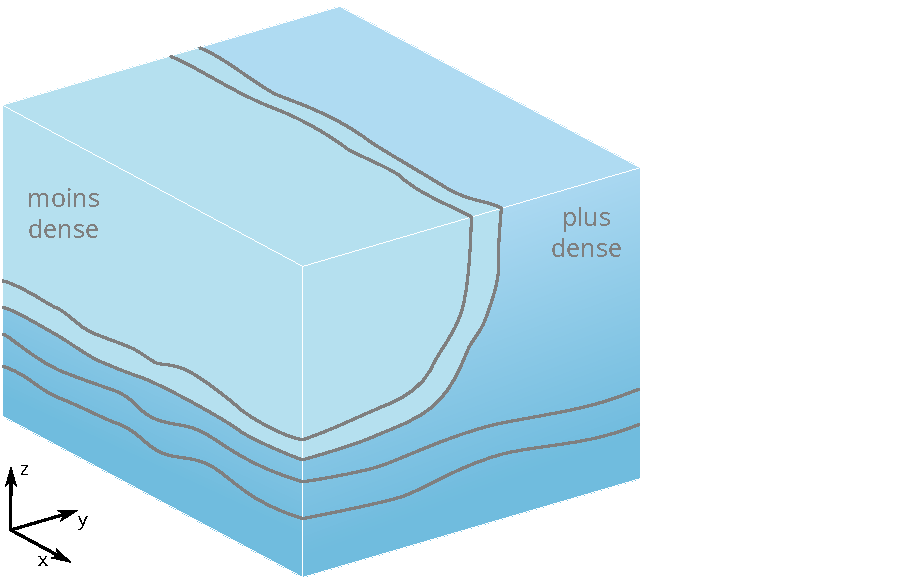
\includegraphics[height=0.8\textheight]{_front_circulation/1.pdf}%
  \llap{\includegraphics<5>[height=0.8\textheight]{_front_circulation/6.pdf}}%
  \llap{\includegraphics<1->[height=0.8\textheight]{_front_circulation/2.pdf}}%
  \llap{\includegraphics<2->[height=0.8\textheight]{_front_circulation/3.pdf}}%
  \llap{\includegraphics<3->[height=0.8\textheight]{_front_circulation/4.pdf}}%
  \llap{\includegraphics<4->[height=0.8\textheight]{_front_circulation/5.pdf}}%
  \llap{\includegraphics<6>[height=0.8\textheight]{_front_circulation/7.pdf}}%
\end{frame}

%% --------------------------------------

\begin{frame}
  \frametitle{Quantification de l'apport de nutriments}

  littérature

\end{frame}

%% --------------------------------------

\begin{frame}
  \frametitle{Déclenchement du bloom}
  \framesubtitle{hypothèse de Sverdrup}
  importance de la profondeur de la couche de mélange

  restratification au printemps

  accompagner d'un schéma ?
\end{frame}

%% --------------------------------------

\begin{frame}
  \frametitle{Modification de la phénologie du bloom}
  seulement dans un modèle (même si forcé par observations)

  \includegraphics[width=0.4\textwidth]{mahadevan_2012_fig3.pdf}
  Mahadevan et al.\ (2012)
\end{frame}

%% --------------------------------------

\begin{frame}
  \frametitle{Région d'étude: autour du Gulf Stream}

  \onslide<1->{plusieurs \strong{biorégions}}
  \onslide<2->{, fronts d'intensités variées}

  \vfill

  \includegraphics[
  width=\textwidth, height=\textheight, keepaspectratio
  ]{zone_separation.pdf}
\end{frame}

%% --------------------------------------

\subsection{Problématiques}

\begin{frame}
  \boxtitle{Problématiques}
  \vspace{2em}

  \begin{enumerate}
    \setlength{\itemsep}{1em}
    \item Quantifier la \emph{réponse de la chlorophylle-a} aux dynamiques \emph{frontales} dans la région du Gulf Stream
    \uncover<2->{\item Influence de la \emph{saison}, du \emph{régime} biogéochimique, et de \emph{l’intensité} des fronts ?}
    \uncover<3->{\item Détecter un \emph{bloom précoce} dans les fronts ?}
  \end{enumerate}
\end{frame}

%% --------------------------------------

\begin{frame}
  \frametitle{Détecter les fronts par satellite}

  \begin{block}{}
    On utilise la \strong{SST} comme proxy de la densité
  \end{block}

  \begin{block}{}
    Plusieurs méthodes existantes:
    \begin{itemize}
            \setlength{\itemsep}{1.2em}
      \item “simple” dérivation: gradient, Sobel, Laplacien, \dots
      \item filtrer auparavant: Canny (1986), Belkin--O'Reilly (2009)
      \item fenêtre glissante: Cayula--Cornillon (1992), Nieto et al. (2012), Miller (2009), \strong{Liu \& Levine (2016)}
    \end{itemize}
  \end{block}
\end{frame}

%% --------------------------------------

\begin{frame}
  \frametitle{Méthode du “Heterogeneity-index”}
  \onslide<1->{Fenêtre glissante}\onslide<2->{, dans laquelle on calcule 3 composantes}
  \\[1em]
  \multigraph[height=0.8\textheight]{4}{zoom_front}

\end{frame}

%% --------------------------------------

\begin{frame}
  \frametitle{Données utilisées: SST}

  \begin{block}{Choisie dans la suite}
    \begin{itemize}
      \item ESA-SST-CCI / C3S
      \item journalières, 4km
      \item L4: interpolation spatiale de multicapteurs IR, pas de nuages
    \end{itemize}
  \end{block}

  \begin{block}{Aussi considérées}
    \begin{itemize}
      \item MODIS projetée à 1km (seulement 2 capteurs, difficile)
      \item Multiscale Ultrahigh Resolution, 1km
      \item Réanalyse Mercator GLORYS, 12km (différences importantes avec autres produits)
    \end{itemize}
  \end{block}

\end{frame}

\begin{frame}
  \frametitle{Données utilisées: Chl-a}

  \begin{block}{Choisie dans la suite}
    \begin{itemize}
      \item Copernicus-Globcolour,
      \item journalières, 4km
      \item L3: multicapteurs, avec nuages
    \end{itemize}
  \end{block}

  \begin{block}{Aussi considérées}
    \begin{itemize}
      \item MODIS projetée à 1km
      \item ESA-OC-CCI / C3S, équivalent
    \end{itemize}
  \end{block}

\end{frame}

%% --------------------------------------

\begin{frame}
  \frametitle{Résultats: Évolution de la Chl-a avec le HI}
  \includegraphics[
  width=\textwidth, height=0.8\textheight, keepaspectratio
  ]{results/chl_vs_hi.pdf}
\end{frame}

\begin{frame}
  \frametitle{Occurence des fronts}
  \includegraphics[
  width=\textwidth, height=0.8\textheight, keepaspectratio
  ]{results/fronts_occurrence.pdf}

  \vfill

  \begin{block}{}

  \end{block}

\end{frame}

\section{Région subtropicale -- Augmentation de la Chlorophylle dans les fronts}
\sectionframe{1}

\section{Région du Gulf-Stream -- Intensité des fronts}
\sectionframe{2}

\section{Région subpolaire -- Phénologie du bloom}
\sectionframe{3}


\begin{frame}
  \frametitle{Chronométrer le bloom: démarrage et durée}
  \multigraph[width=\textwidth, height=0.8\textheight, keepaspectratio]{9}{phenologie_méthode}
\end{frame}

%% --------------------------------------

\begin{frame}
  \frametitle{Différences de phénologie entre background et fronts}
  \multigraph[width=\textwidth, height=0.8\textheight, keepaspectratio]{4}{phenologie_lag}
\end{frame}

%% --------------------------------------

\begin{frame}
  \frametitle{Décalage du \emph{\textit{démarrage}} du bloom}
  \multigraph[width=0.85\textwidth]{7}{bloom}

  \vfill

  \begin{overlayarea}{\textwidth}{2\baselineskip}
    \only<6->{fit pour les fronts faibles: \(-6.7 \pm 1.1\) jours}

    \only<7->{fit pour les fronts forts: \(-13.5 \pm 1.5\) jours}
  \end{overlayarea}
\end{frame}

%% --------------------------------------

\begin{frame}
  \frametitle{Décalage de la \emph{\textit{durée}} du bloom}
  \includegraphics[
  width=0.90\textwidth, height=0.7\textheight,
  keepaspectratio]{durée_bloom.pdf}

  \vfill

  Blooms plus \emph{longs} dans les \emph{fronts}, mais moins significatif
\end{frame}

%% --------------------------------------

\section{Conclusions}

\begin{frame}
  \frametitle{Conclusions}

\end{frame}

%% --------------------------------------

\section{Perspectives}
\begin{frame}
  \frametitle{Perspectives}

  \begin{itemize}
    \item vers le global
    \item vers les PFT (plus que déjà?)
    \item nécessité de développer outils de détection de fronts
  \end{itemize}

\end{frame}

%% --------------------------------------

\begin{frame}
  Fin
\end{frame}

\end{document}
